Pingo ist eine Software-Lösung, die bereits seit dem Jahr 2011 an der Universität Paderborn entwickelt wird. Der Name ist ebenfalls ein Akronym und steht für „\textbf{P}eer \textbf{In}struction for Very Large \textbf{G}r\textbf{o}ups“. Im Gegensatz zu StuReSy ist Pingo bereits weiter verbreitet und wird an vielen deutschen Hochschulen eingesetzt. Dahinter steht außerdem ein ganzes Team von akademischen Mitarbeitern. Seit 2019 wird Pingo von der universitätsnahen Coactum GmbH betrieben und weiterentwickelt.\newline

Prinzipiell handelt es sich bei Pingo um eine reine Web-Applikation, die öffentlich und kostenlos unter www.trypingo.com zugänglich ist. Für die Nutzung muss jedoch ein Benutzerkonto eröffnet werden. Pingo steht unter einer Open-Source-Lizenz und somit können Nutzer auch eine eigene Pingo-Instanz betreiben. Pingo ist in der Programmiersprache Ruby und mithilfe des Web-Frameworks „Ruby on Rails“ implementiert worden.

Bei den unterstützten Fragetypen sind beide Programme nahezu identisch: Single Choice, Multiple Choice, Freitext und numerische Fragen sind möglich.


Pingo hat prinzipiell einen sehr großen Funktionsumfang, jedoch fehlen entscheidende Funktionen für den Einsatz in der Programmierlehre:
\begin{itemize}
    \item \textbf{Keinerlei Formatierungs-Möglichkeiten}: Fragen innerhalb der Pingo-Plattform können überhaupt nicht formatiert werden. Damit können weder Fettschreibungen, Unterstreichungen oder Zeilenumbrüche verwendet werden. Dementsprechend ist auch die übersichtliche Darstellung von Quelltext vollkommen unmöglich.
\end{itemize}

\begin{figure}[H]
    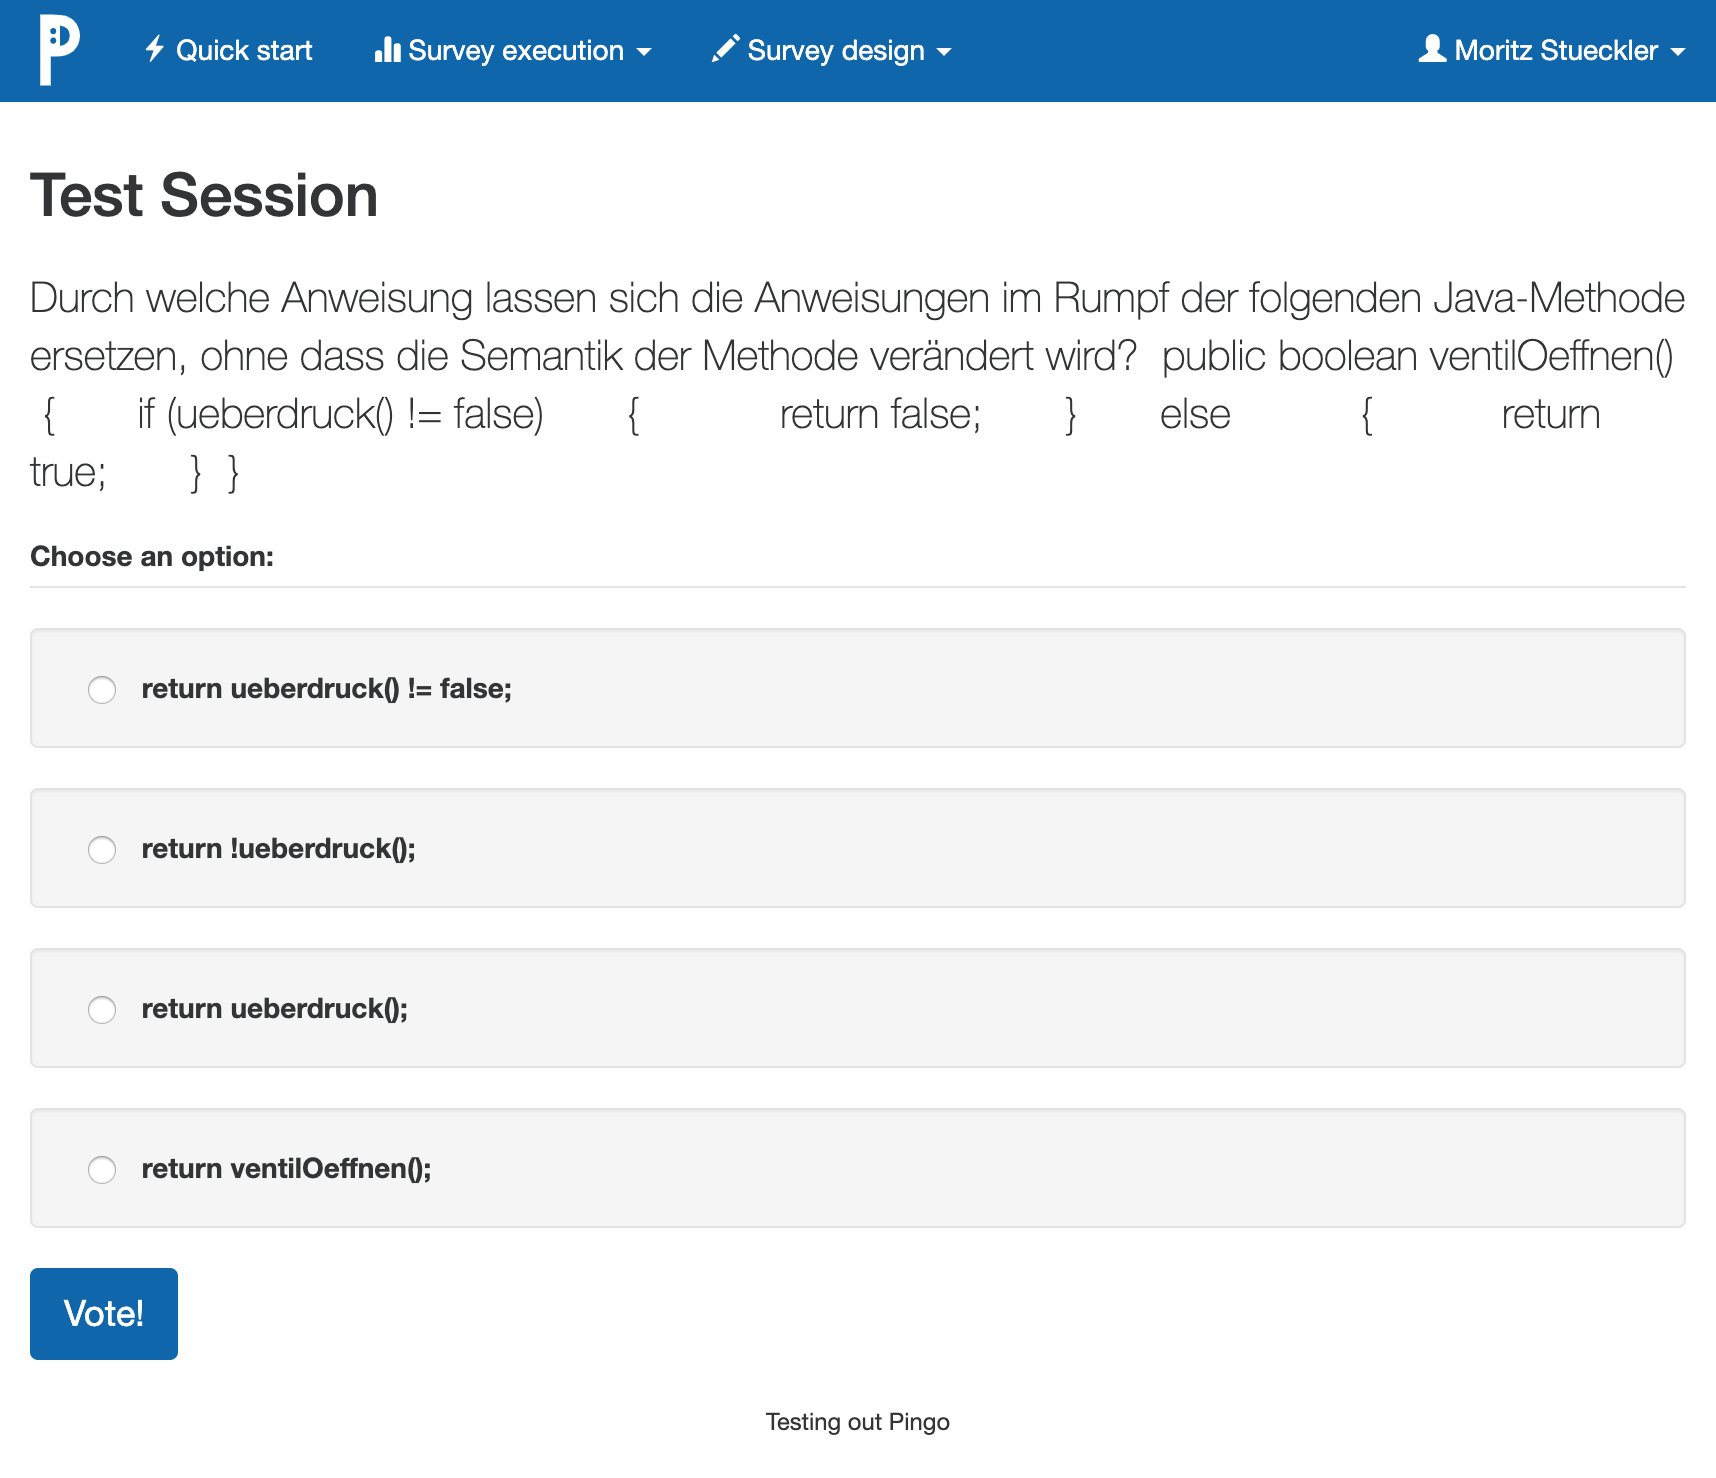
\includegraphics[width=12cm]{chapter/bewertung/bilder/pingo_problem1.png}
    \centering
    \caption{Pingo verfügt über keinerlei Text-Formatierungsoptionen und ist daher ungeeignet für die Darstellung von Quelltext.}
    \label{Abbildung 2.4}
\end{figure}